%&latex
\documentclass[letterpaper,11pt]{article}
\usepackage{graphicx}
\usepackage[margin=1.0in]{geometry}
\usepackage[hyphens]{url}
\usepackage{hyperref}

\makeatletter
\setlength{\@fptop}{0pt}
\makeatother

\title{BAMSurgeon: Methods for spike-in mutations on BAM files}
\author{Adam D. Ewing (adam.ewing@mater.uq.edu.au)}
\begin{document}
 \date{May 22, 2014}
 \maketitle

\section{Introduction}
\subsection{Software Dependencies}
BAMSurgeon requires the following software packages be available:

\begin{enumerate}
  \item samtools/wgsim/tabix (\url{http://samtools.sourceforge.net/})
  \item pysam (\url{http://code.google.com/p/pysam/} or \texttt{pip install pysam})
  \item bwa (\url{http://bio-bwa.sourceforge.net/})
  \item velvet (\url{http://www.ebi.ac.uk/~zerbino/velvet/})
  \item exonerate (\url{http://www.ebi.ac.uk/~guy/exonerate/})
  \item picard (\url{http://http://picard.sourceforge.net/})
\end{enumerate}

\subsection{How to (f$\vert$m)ake a tumour}
One of the primary use cases for BAMSurgeon is to test somatic mutation calling methods, so we have provided an outline of how this can be accomplished (Fig 1). Suggestions for improvements to the process are welcome. There are three stages to this process:
\begin{enumerate}
\item Preprocessing (BAM selection and splitting)
\item Mutating (selecting mutation sites, running BAMSurgeon, generating ``truth'' VCFs)
\item Postprocessing (BAM repair, GATK IndelRealigner, BQSR)
\end{enumerate}

\paragraph{1. Preprocessing}
TODO

\paragraph{2. Mutating}
TODO

\paragraph{3. Postprocessing}
TODO

\subsection{Known bugs and limitations}
BAMSurgeon is under rapid development driven by suggesting and bug reports from the mutation calling community.



\section{Adding SNVs to existing BAM alignments (addsnv)}
\subsection{Usage}
\begin{verbatim}
usage: addsnv.py [-h] -v VARFILENAME -f BAMFILENAME -r REFFASTA -o OUTBAMFILE
                 [-s SNVFRAC] [-m MUTFRAC] [-n NUMSNVS] [-c CNVFILE]
                 [-d COVERDIFF] [-p PROCS] [--samtofastq SAMTOFASTQ]
                 [--mindepth MINDEPTH] [--nomut] [--det] [--force] [--single]
                 [--maxopen MAXOPEN] [--requirepaired] [--skipmerge]
                 [--bwamem]

adds SNVs to reads, outputs modified reads as .bam along with mates

optional arguments:
  -h, --help            show this help message and exit
  -v VARFILENAME, --varfile VARFILENAME
                        Target regions to try and add a SNV, as BED
  -f BAMFILENAME, --bamfile BAMFILENAME
                        sam/bam file from which to obtain reads
  -r REFFASTA, --reference REFFASTA
                        reference genome, fasta indexed with bwa index -a
                        stdsw _and_ samtools faidx
  -o OUTBAMFILE, --outbam OUTBAMFILE
                        .bam file name for output
  -s SNVFRAC, --snvfrac SNVFRAC
                        maximum allowable linked SNP MAF (for avoiding
                        haplotypes) (default = 1)
  -m MUTFRAC, --mutfrac MUTFRAC
                        allelic fraction at which to make SNVs (default = 0.5)
  -n NUMSNVS, --numsnvs NUMSNVS
                        maximum number of mutations to try (default: entire
                        input)
  -c CNVFILE, --cnvfile CNVFILE
                        tabix-indexed list of genome-wide absolute copy number
                        values (e.g. 2 alleles = no change)
  -d COVERDIFF, --coverdiff COVERDIFF
                        allow difference in input and output coverage
                        (default=0.9)
  -p PROCS, --procs PROCS
                        split into multiple processes (default=1)
  --samtofastq SAMTOFASTQ
                        path to picard SamToFastq.jar
  --mindepth MINDEPTH   minimum read depth to make mutation
  --avoidreads AVOIDREADS
                        file of read names to avoid (mutations will be skipped
                        if overlap)

  --nomut               dry run
  --det                 deterministic base changes: make transitions only
  --force               force mutation to happen regardless of nearby SNP or
                        low coverage
  --single              input BAM is single-ended (default is paired-end)
  --maxopen MAXOPEN     maximum number of open files during merge (default
                        1000)
  --requirepaired       skip mutations if unpaired reads are present
  --skipmerge           final output is tmp file to be merged
  --bwamem              realignment with BWA MEM (instead of backtrack)

\end{verbatim}

\subsection{Description}
    Single nucleotide changes are introduced to an existing BAM alignment using \texttt {addsnv.py} as outlined in Figure 2. Input consists of a list of locations where SNVs will be made, a target BAM alignment, and a reference genome indexed using bwa (preferably the same genome used to align the reads in the BAM file). 

\subsection{Input}
\paragraph{Mutation input (-v/--varfile)}
	Input to addsnv.py (-v/--varfile) is BED-3 format plus an extra optional column for the desired variant allele fraction (VAF). The default VAF is specified via -m/--mutfrac. For example:
\begin{verbatim}
22 34166720 34166720 0.25
22 33908770 33908770 0.15
22 33714964 33714964 0.5
22 33769483 33769483 0.75
22 33958087 33958087 0.01
22 34264774 34264774 0.25
22 33702084 33702084 0.2
22 34141184 34141184
22 33926586 33926586
22 33943910 33943920
\end{verbatim}

    The above input will cause addsnv to attempt 10 SNVs at the specified locations, using the VAF specified in the fourth column if available, otherwise defaulting to 0.5 or whatever is specified by -m/--mutfrac (e.g. the last three lines). Note that the positions in the last input line define a region 10bp wide rather than a specific position as in the first 9 lines. When specified this way, addsnv will choose one of the 10 possible positions at random. 

\paragraph{BAM Alignment input (-f/--bamfile)}
	BAMs ideally should adhere to SAM specification i.e. they should validate via picard\'s ValidateSamFile. BAMs should be sorted in coordinate order and indexed. BAMs should consist either of entirely paired-end reads or entirely single-end (fragment) reads using the --single option, mixing paired and single reads yields unpredictable results. Currently, bwa backtrack (\texttt{bwa aln}) and bwa mem are supported, although it should be straightforward enough to add further aligners through modification of the \texttt{remap\_paired} function. In practice we have been able to spike mutations into RNA-seq MapSplice BAMs, for instance.

\paragraph{Reference genome (-r/--reference)}
	The reference genome should be the \textbf{same as that used to create the target BAM file}, specifically the chromosome names and lengths in the reference FASTA must be the same as in the BAM header. The reference must be indexed for bwa (\texttt{bwa index}) and indexed with samtools (\texttt{samtools faidx}).
	
\paragraph{Avoiding existing SNPs with -s/--snpfrac (optional, default=1.0)}
	In an attempt to preserve haplotype structure and avoid confusion by spiking mutations on top of existing heterozygous alleles, the -s/--snpfrac cutoff may be useful. For a selected mutation site $S$ and specified cutoff $f$ starting from the leftmost base $L$ of the leftmost read containing $S$ and ending at the rightmost base $R$ of the rightmost read containing $S$, the minor allele frequency $M$ for every intervening base is calculated for every base in the interval $[L,R]$. If $M < f$ for all bases in $[L,R]$ the mutation at $S$ is allowed, and skipped otherwise. Note, do not confuse this with -m/--mutfrac, which is the target variant allele frequency for mutations unless overridden in the mutation input file. By default this function is turned off (threshold minor allele frequency set to 1.0). Setting this too low can yield few successful mutations as sequence errors will inhibit successful spike-in, we recommend a setting of 0.1 for Illumina GA/HiSeq reads.

\paragraph{CNV file (-c/--cnvfile) (optional)}
	It is possible to simulate adding mutations to a single haplotype for copy-number variant regions. For example, if a region has absolute copy number 3 (instead of 2), a mutation into one haplotype should have an apparent VAF of roughly 0.33 instead of 0.5. This optional file should be in BED-3 format plus a fourth column representing the absolute copy number for the region defined by the chromosome/contig, start, and end fields. The genome is assumed to be diploid thus an absolute copy number of 2 will not adjust the variant allele fractions. Absolute copy numbers below 2 will adjust VAFs higher and absolute copy numbers above 2 will adjust VAFs correspondingly lower.

\paragraph{Additional options}
\begin{itemize}
\item -d/--coverdiff : threshold on output coverage divided by input coverage for mutation sites. Mutations can cause alignments to change, if this is undesired set this high, if this is part of the fun, set this low.
\item -p/--procs : BAMSurgeon programs currently spawn a new process for each spikein, to speed things along the processes can be run concurrently with the number of simultaneous jobs set by this parameter.
\item --samtofastq : path to SamToFastq.jar provided by picard tools, this is required for the --bwamem option
\item --mindepth : minimum depth at sites for mutations, sites with fewer reads in pileup column will be dropped. Default is 5 reads.
\item --avoidreads : addsnv and addindel can be passed a list of read names to avoid when making mutations. Any sites selected that overlap these reads will be dropped. This feature exists as a means to ensure mutations across multiple runs do not overlap.
\item --force : force the addition of a mutation even if it fails thresholds set by --mindepth and -c/--coverdiff. Not recommended for most use cases.
\item --single : covered above, assume reads are single-end (i.e. fragment reads).
\item --maxopen : set the maximum number of open files (check your system limit with \texttt{ulimit -a})
\item --requirepaired : drop mutations where a paired end in the region cannot be located. However, it is probably better to correct the problem in the BAM file than to resort to using this option.
\item --skipmerge : instead of replacing the mutated and realigned reads back into the original BAM, which is normally the final step, leave the addsnv.
\item --bwamem : realign reads using bwa mem. The target BAM file should have also been aligned using bwa mem if this option is used.
\item options not listed here are either brand new and the manual has not been updated as yet, or they are there for debugging and will be removed in the future.
\end{itemize}


\section{Adding INDELs to existing BAM alignments (addindel)}
\subsection{Usage}
\begin{verbatim}
usage: addindel.py [-h] -v VARFILENAME -f BAMFILENAME -r REFFASTA -o
                   OUTBAMFILE [-s SNVFRAC] [-m MUTFRAC] [-n NUMSNVS]
                   [-c CNVFILE] [-d COVERDIFF] [-p PROCS]
                   [--samtofastq SAMTOFASTQ] [--mindepth MINDEPTH] [--nomut]
                   [--det] [--force] [--single] [--maxopen MAXOPEN]
                   [--requirepaired] [--bwamem] [--skipmerge]

adds SNVs to reads, outputs modified reads as .bam along with mates

optional arguments:
  -h, --help            show this help message and exit
  -v VARFILENAME, --varfile VARFILENAME
                        Target regions to try and add a SNV, as BED
  -f BAMFILENAME, --bamfile BAMFILENAME
                        sam/bam file from which to obtain reads
  -r REFFASTA, --reference REFFASTA
                        reference genome, fasta indexed with bwa index -a
                        stdsw _and_ samtools faidx
  -o OUTBAMFILE, --outbam OUTBAMFILE
                        .bam file name for output
  -s SNVFRAC, --snvfrac SNVFRAC
                        maximum allowable linked SNP MAF (for avoiding
                        haplotypes) (default = 1)
  -m MUTFRAC, --mutfrac MUTFRAC
                        allelic fraction at which to make SNVs (default = 0.5)
  -n NUMSNVS, --numsnvs NUMSNVS
                        maximum number of mutations to try (default: entire
                        input)
  -c CNVFILE, --cnvfile CNVFILE
                        tabix-indexed list of genome-wide absolute copy number
                        values (e.g. 2 alleles = no change)
  -d COVERDIFF, --coverdiff COVERDIFF
                        allow difference in input and output coverage
                        (default=0.1)
  -p PROCS, --procs PROCS
                        split into multiple processes (default=1)
  --samtofastq SAMTOFASTQ
                        path to picard SamToFastq.jar
  --mindepth MINDEPTH   minimum read depth to make mutation
  --avoidreads AVOIDREADS
                        file of read names to avoid (mutations will be skipped
                        if overlap)

  --nomut               dry run
  --det                 deterministic base changes: make transitions only
  --force               force mutation to happen regardless of nearby SNP or
                        low coverage
  --single              input BAM is simgle-ended (default is paired-end)
  --maxopen MAXOPEN     maximum number of open files during merge (default
                        1000)
  --requirepaired       skip mutations if unpaired reads are present
  --bwamem              realignment with BWA MEM (instead of backtrack)
  --skipmerge           final output is tmp file to be merged

\end{verbatim}

\subsection{Description}
Short insertions and deletions (commonly referred to as INDELs) can be added to BAM files using addindel.py. The options are essentially the same as for addsnv.py, but the syntax of the input file is slightly different:

\begin{verbatim}
22 33694303 33694304 0.50 INS ATGGC
22 33815273 33815274 0.25 INS CG
22 33920490 33920491 0.33 INS ATTTGCTTAGCTGAGGGCTTAGGCTTAGCATGCGTA
22 33944542 33944543 0.50 DEL
22 34006643 34006653 0.50 DEL
22 33958087 33958090 0.40 DEL
\end{verbatim}

The first four columns are the same as for addsnv.py input but the fourth column (VAF) is manditory. The fifth column must be either 'INS' or 'DEL' (for insertion or deletion). For insertions there must be a sixth column specifying the sequence to be inserted at the position indicated in the second column (the position in the third column does not matter for insertions). In the above example, the first three columns direct addindel.ppy to (1) add an insertion of ``ATGGC'' at chromosome 22 position 33694303 with 50\% VAF, (2) add an insertion of ``CG'' at position 338152273 with 25\% VAF, and (3) add an insertion of ``ATTTGC...'' with 33\% VAF.

For deletions, the sequence from the start to the end (columns two and three) is deleted. Lines 4,5, and 6 above indicate deletions of 1 bp, 10bp, and 3 bp, respectively.

\section{Adding SVs to existing BAM alignments (addsv.py)}

\subsection{Usage}
\begin{verbatim}
usage: addsv.py [-h] -v VARFILENAME -f BAMFILENAME -r REFFASTA -o OUTBAMFILE
                [-l MAXLIBSIZE] [-k KMERSIZE] [-s SVFRAC]
                [--maxctglen MAXCTGLEN] [-n MAXMUTS] [-c CNVFILE]
                [--ismean ISMEAN] [--issd ISSD] [-p PROCS] [--inslib INSLIB]
                [--delay DELAY] [--nomut] [--noremap] [--noref] [--recycle]
                [--bwamem] [--skipmerge]

adds SNVs to reads, outputs modified reads as .bam along with mates

optional arguments:
  -h, --help            show this help message and exit
  -v VARFILENAME, --varfile VARFILENAME
                        whitespace-delimited target regions to try and add a
                        SNV: chrom,start,stop,action,seqfile (if
                        insertion),TSDlength (if insertion)
  -f BAMFILENAME, --sambamfile BAMFILENAME
                        sam/bam file from which to obtain reads
  -r REFFASTA, --reference REFFASTA
                        reference genome, fasta indexed with bwa index -a
                        stdsw _and_ samtools faidx
  -o OUTBAMFILE, --outbam OUTBAMFILE
                        .bam file name for output
  -l MAXLIBSIZE, --maxlibsize MAXLIBSIZE
                        maximum fragment length of seq. library
  -k KMERSIZE, --kmer KMERSIZE
                        kmer size for assembly (default = 31)
  -s SVFRAC, --svfrac SVFRAC
                        allele fraction of variant (default = 1.0)
  --maxctglen MAXCTGLEN
                        maximum contig length for assembly - can increase if
                        velvet is compiled with LONGSEQUENCES
  -n MAXMUTS            maximum number of mutations to make
  -c CNVFILE, --cnvfile CNVFILE
                        tabix-indexed list of genome-wide absolute copy number
                        values (e.g. 2 alleles = no change)
  --ismean ISMEAN       mean insert size (default = estimate from region)
  --issd ISSD           insert size standard deviation (default = estimate
                        from region)
  -p PROCS, --procs PROCS
                        split into multiple processes (default=1)
  --inslib INSLIB       FASTA file containing library of possible insertions,
                        use INS RND instead of INS filename to pick one
  --delay DELAY         time delay between jobs (try to avoid thrashing disks)
  --nomut               dry run
  --noremap             dry run
  --noref               do not perform reference based assembly
  --recycle
  --bwamem              realign with bwa mem (original shuld be aligned with
                        mem as well!)
  --skipmerge


\end{verbatim}

\subsection{Description}
   Larger structural variants (insertions, deletions, duplications, inversions, and compound rearrangements) are added to existing BAM alignments using \texttt{addsv.py} as described in Figure 3. Input consists of a list of regions where SVs will be made along with a specification of each variant, and as with addsnv and addindel, a target BAM alignment, and a reference genome indexed using bwa are required.

\subsection{Input}
    The input mutation list consists of four columns: chromosome, start of region, end of region, and a controlled-vocabulary description of the mutation. A mutation will not be made if the largest contig obtained from local assembly of the specified region is less than 3 times the maximum expected library size (specified by \texttt{-l/--maxlibsize}). The mutation description starts with either \texttt{INS, DEL, DUP}, or \texttt{INV} for insertion, deletion, duplication, and inversion, respectively and is followed by mutation-specific options. An example follows.

\begin{verbatim}
22 33871043 33884754 DEL 0.9
22 33971043 33984754 INS myseq.fa
22 34071043 34084754 INV
22 34171043 34184754 INS ACTATCGTGGGCTTATGGCTTAGCATTACGGTTATTTTTGCACTGATCGCGGGGGCTACATCATTCATGCTATTACTTGCGTATCGTA
22 34271043 34284754 DUP 3
22 34371043 34384754 INS RND
\end{verbatim}

    For insertions, \texttt{INS} should be followed by either a FASTA file containing the sequence to be inserted, by the nucleotide sequence itself, or by RND if a library of potential insertion sequences is passed in FASTA format via the --inslib option. For example, \texttt{INS ATG} would insert the sequence \texttt{``ATG''} in the middle of the largest contig obtained from the specified region, while \texttt{INS LINE1.fa} would insert the sequence in the FASTA-formatted file \texttt{LINE1.fa} into the largest contig. For deletions, \texttt{DEL} should be followed by the fraction of the largest contig to be deleted, where 1.0 indicates a deletion of the largest assembled region minus one library length on each end. e.g. {DEL 0.5}. Inversions (\texttt{INV}) have no further options - the region inside the largest contig will be inverted. Duplications (\texttt{DUP}) have one optional parameter, an integer specifying the number of times the sequence of the largest contig should be duplicated, e.g. \texttt{DUP 2} specifies the region is duplicated twice. In general, we recommend that short insertions and deletions (those shorter than one read length) be created with addindel.py instead of addsv.py as addindel.py does not require reconstruction of the region through sequence assembly and is thus less error-prone.

    Compound variants are also possible by chaining a number of mutations together in a comma-delimited list, e.g. \texttt{DUP 1, DEL 0.5, INS AAATCC, INV} would duplicate the region inside the largest contig once, delete half the width of the region, insert the sequence \texttt{AAATCC}, and invert the region. Good luck!

\subsection{Output}
    Where mutations add sequence (e.g. duplications), new reads are created that will be added to the original BAM, and where mutations remove sequence (e.g. deletions) those reads are maked as excluded (excluded read names are recorded in the file specified by \texttt{-x/--excluded}). Excluded reads are not carried over from the original BAM to the mutated BAM, creating the copy number effect associated with deletion.
    
     Output consists of a BAM file containing the spike-in mutations and a directory of log files describing which bases were changed in which reads (one log per mutation) and the local assemblies for each region where a mutation was made. Currently, the directory containing output logs for SV spike-ins can be transformed into VCF format using the script \texttt {makevcf\_sv.py} in the \texttt {etc/} subdirectory. The spike-in process may be done concurrently through the use of the \texttt {-p/--procs} option. Here are some extended descriptions for additional options not mentioned yet:
     
\begin{itemize}
\item -s/--snvfrac : equivalent to -m/--mutfrac for addindel.py and addsnv.py (will fix)
\item -k/--kmer : kmer size to be fed to velvet, which is used for assembly
\item -n : only attempt this many mutations
\item --ismean/--issd : the mean and standard deviation of the library size should be estimated from the original bam and specified through these arguments. This can be accomplished a number of ways, I suggest CollectInsertSizeMetrics from the picard tools.
\item --inslib : a FASTA file can be specified and insertions can be tagged with RND instead of a sequence or file. If this is done, a sequence will be chosen at random from the FASTA file specified by --inslib and inserted.
\item --bwamem : as with other scripts, use bwa mem instead of the default which is bwa backtrack
\item --skipmerge : same meaning as for addsnv/addindel
\end{itemize}

\newpage % forces fig 1 into the right place
\begin{figure}[!h]
\centering
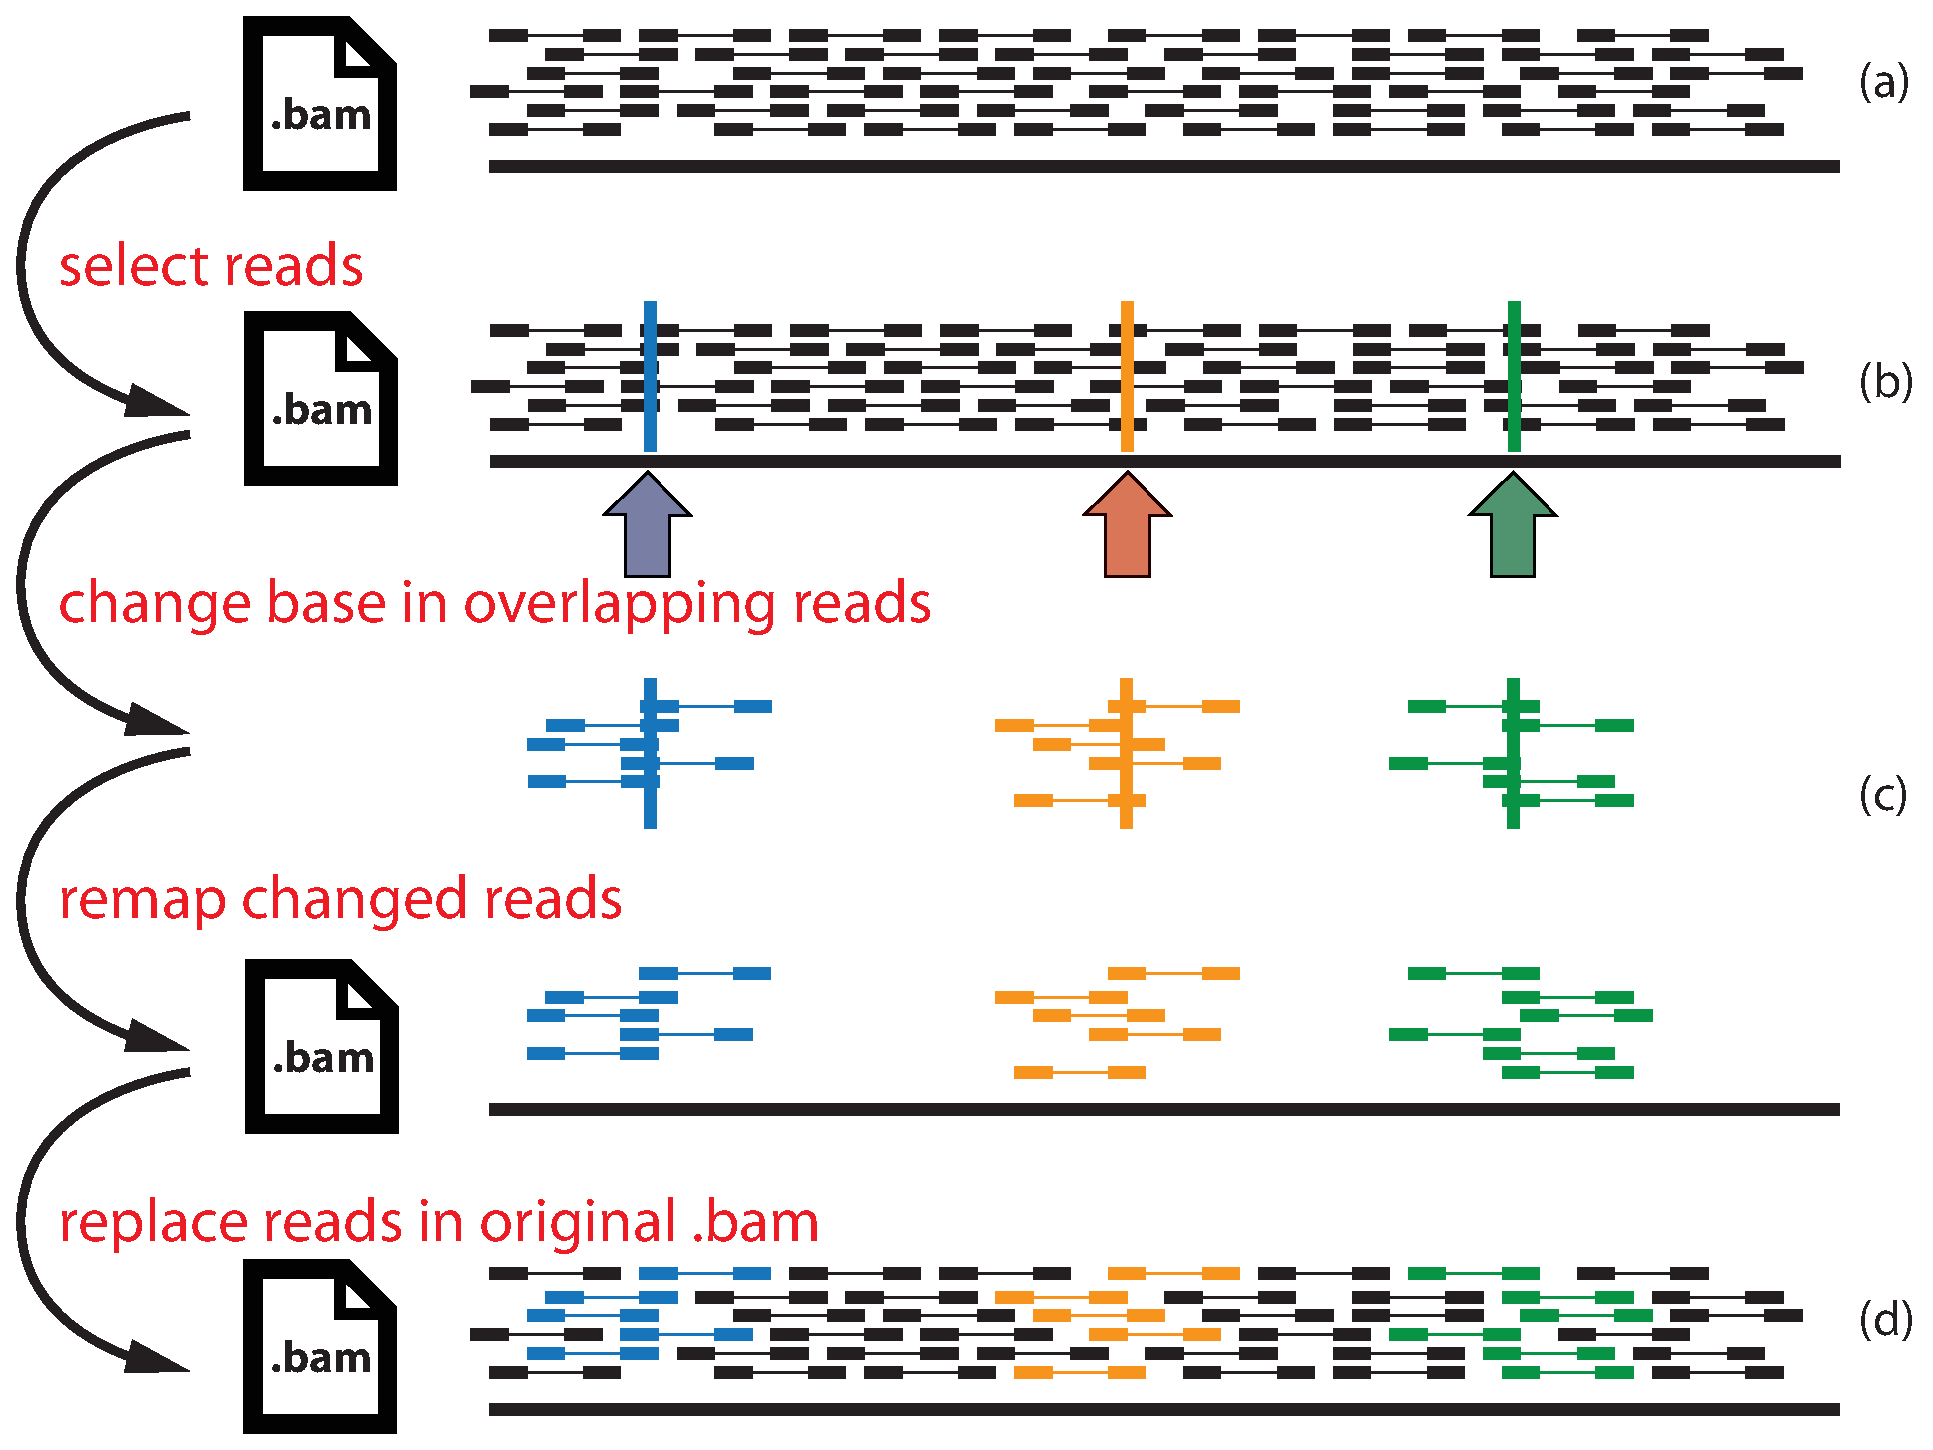
\includegraphics[width=5.5in]{bamsurgeon_snv.eps}
\caption{Method for adding SNVs to existing BAM alignments. Starting with the original BAM alignment (a) and a list of positions (b), reads overlapping the chosen positions are selected the target base change is made (c). Altered reads are re-mapped the the reference genome using bwa, and the modified, realigned reads replace the unmodified versions in the original BAM (d).}
\end{figure}

\newpage % forces fig 2 into the right place

\begin{figure}[!h]
\centering
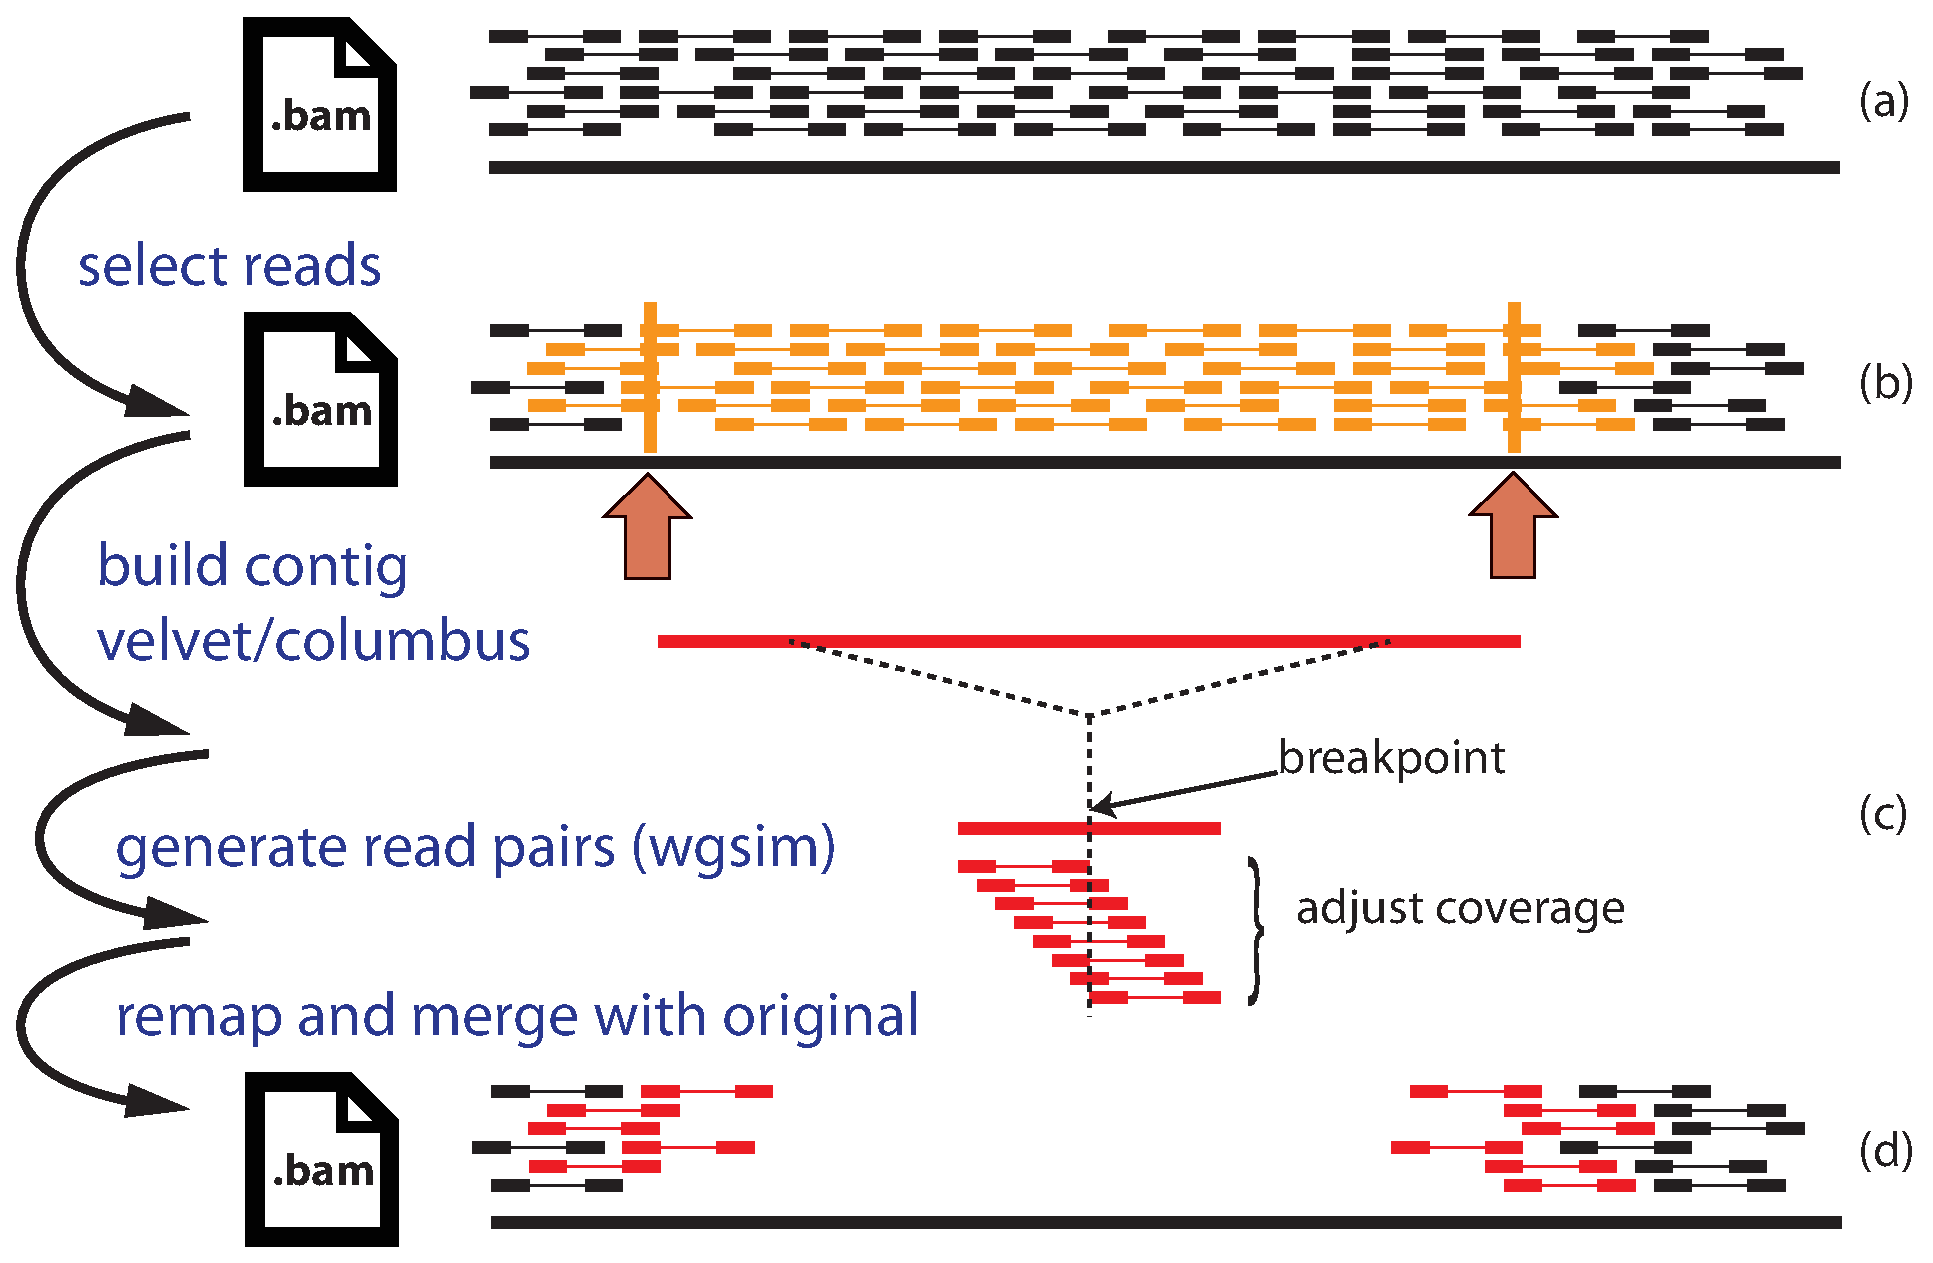
\includegraphics[width=5.5in]{bamsurgeon_sv_del.eps}
\caption{Method for adding multi-nucleotide variants (indels and SVs) to existing BAMs: deletion example. Starting with the original BAM alignment (a) regions, e.g. (b), are assembled using Velvet/Columbus (\texttt{http://www.ebi.ac.uk/~zerbino/velvet/}) and the desired mutation(s) are created in the largest contig. Read coverage is simulated over the contig using wgsim (\texttt{https://github.com/lh3/wgsim}, also included with samtools) with parameters \texttt{-e 0 -r 0 -R 0} to suppress additional mutations, other parameters are set based on the input BAM and desired coverage. Simulated coverage is scaled based on whether the mutation is adds sequence (duplication) or removes sequence (deletions), and replaced into the original BAM while excluded reads are removed from the original BAM (d).}
\end{figure}

\section{Testing}
The \texttt{test/} directory contains scripts useful for testing bamsurgeon installations, one for SNVs and one for SVs.
\subsection{Testing addsnv.py}
The script {test/test\_snv.sh} may be run with no parameters to display a usage statement:
\begin{verbatim}
usage: ./test_snv.sh <number of SNPs> <number of threads> <reference indexed with bwa index>
\end{verbatim}

The number of SNPs can be up to 100 and are selected from the file \texttt{test\_data/random\_snvs.txt}, number of threads must be specified, use 1 to run on a single core, and the final argument must be a path to a human genome (GRCh37) reference indexed with \texttt{bwa index -a bwtsw}. The reference \textbf{should not} use the 'chr' prefix on the chromosome names.

\subsection{Testing addindel.py}
The script {test/test\_sv.sh} may be run with no parameters to display a usage statement:
\begin{verbatim}
usage: ./test_indel.sh <number of threads> <reference indexed with bwa index>
\end{verbatim}

\subsection{Testing addsv.py}
The script {test/test\_sv.sh} may be run with no parameters to display a usage statement:
\begin{verbatim}
usage: ./test_sv.sh <number of threads> <reference indexed with bwa index>
\end{verbatim}



\section{Other Considerations}
\subsection{System Requirements}
For each process (specified by -p/--procs) add*.py will require ~4GB RAM. So for 8 concurrent mutation processes, you should have 32GB RAM. System requirements may decrease in the future as we find ways to improve efficiency.

\subsection{Alignments}
Reads should be re-aligned using the same aligner and parameters as were used to create the original BAM file. By default, bamsurgeon assumes alignments were performed using bwa aln with parameters \texttt{-q 5 -l 32 -k 3 -o 1}. The specific parameters are not currently specifiable on the command line but may be altered through modification of the functions \texttt{remap\_paired} (for paired reads) or \texttt{remap\_single}.

\section{Acknowledgements}
We would like to thank everyone who has submitted a pull request or bug report through github, the synapse forums for the DREAM Somatic Mutation Calling challenge, or by other means.

\end{document}
